\chapter[図の貼り方および表,式の書き方]{図の貼り方および\\表,式の書き方 }

\section{図の貼り方}
\seclabel{fig}

\subsection{基本的な図の貼り方}
図を貼る際には例えば以下のようにする.
\begin{figure}[t]%
  \begin{center}%
    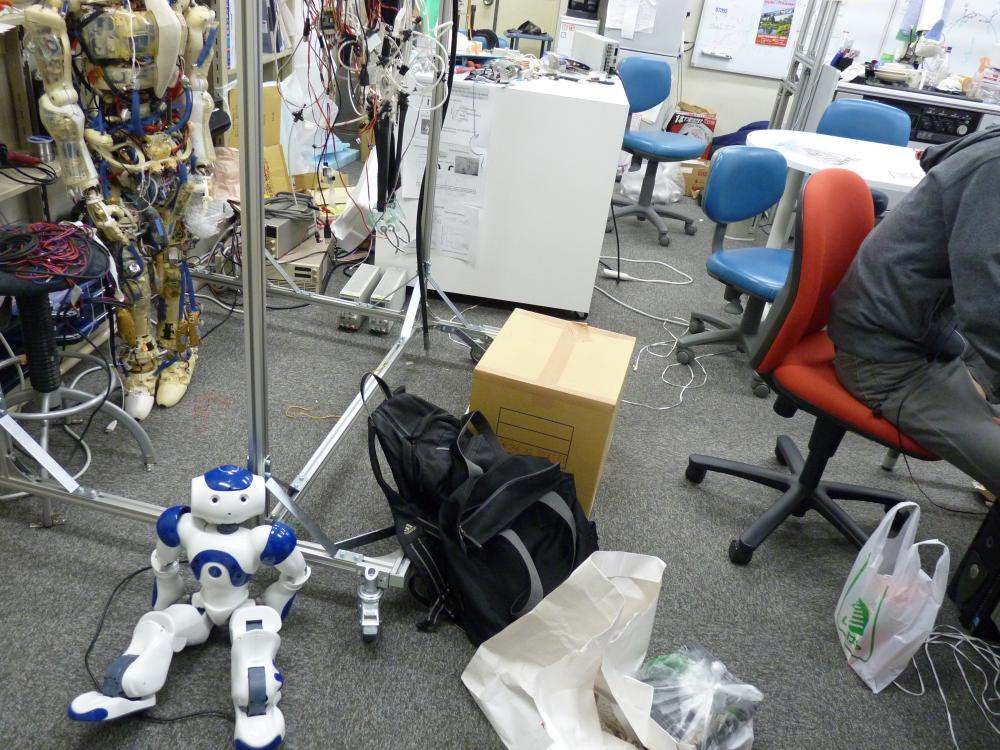
\includegraphics[width=0.50\hsize]{\FIGDIR/photo.jpg}%
    \caption{図の貼り方}%
    \label{fig:lab}%
  \end{center}%
\end{figure}%
図\ref{fig:lab}はこのようにして貼られた図である.
図に対して言及するときはこのようにrefコマンドを使う.
refコマンドの引数を,図を貼った時のコマンド群中のlabelコマンドの引数と対応させることで,意図した図に対してrefすることができるのである.

さて,先ほどの図の貼り方はちょっとめんどくさい.
大体,たかが図を一枚貼るためにこんな数行使った処理をいちいち書いてられないし,ソースコードのスペース的にもたくさん消費してしまってアホみたいである.
そのあたりを解決するのが,figコマンドである.
(figコマンドはいわば自作関数で,ikuo.styの中に定義されている.)
figコマンドを使うと,下記のように図を貼ることができる.
\fig{photo.jpg}{width=.50\hsize}{figコマンドを使って貼った図}
\figref{photo.jpg}はfigコマンドを使って貼った図である.
そして,今,気づいただろうか.
今のrefはただのrefではなく,figrefコマンドを使ってrefを行ったものである.
(figrefコマンドもfigコマンド同様にikuo.styの中で定義されている.)
figrefコマンドを使うと,いちいち「図」とか「fig.」とかをrefコマンドの前に書く必用がなくなり,便利である.
更に,「図」でなく「fig.」として参照するように変更する必用が生じた時にも,ikuo.styの中のfigrefコマンドの定義箇所にて変更をするだけで文書全体に変更が行われるのでとても有用であり,figrefコマンドを使わないのは愚かしい行為である.


\subsection{figに関連する便利コマンド}

figコマンドには残念ながら,図の位置を指定する引数が存在しない.
figコマンドの定義を見ると,位置指定オプションは[tbp]となっており,ページ上端,下端,まるまる1ページ,という優先度で位置が指定されることがわかる.
どうしてもページ下端に図を貼りたいんだ,という時にはfigbコマンドが用意されている.
\figb{photo2.jpg}{width=.50\hsize}{figbコマンドを使って貼った図}
\figref{photo2.jpg}はfigbコマンドを使って貼った図である.

どうしても位置を自分で指定したい,という場合はfigposコマンドを使う.
figposコマンドは第4引数が位置指定オプションに反映されるため,下記のように使うことができる.
\figpos{photo3.jpg}{width=.50\hsize}{figposコマンドを使って貼った図}{t}
\figref{photo3.jpg}はfigposコマンドを使って貼った図である.

上記各コマンドと合わせ,定義されているfig関連のコマンドを以下にまとめておく.
\begin{itemize}
\item fig\\
  図を貼るときに使う一番基本的なコマンド.
  位置指定は[tbp]となる.
  
\item twofigs\\
  2枚の図を立てに並べて貼るときに使うコマンド.
  キャプションは1つだけつき,ラベルは最初の図のファイル名になる.
  位置指定は[tbp]となる.
  
\item figthroug\\
  複数段組の文書中で,段組をぶちぬいて図を貼るときに使うコマンド.
  
\item figb\\
  ページ下端に図を貼るときに使うコマンド.
  
\item figpos\\
  任意の位置を指定して図を貼るときに使うコマンド.
  
\item doublefig\\
  2枚の図を横に並べて貼るときに使うコマンド.
  キャプションは1つだけつき,ラベルは最初の図のファイル名になる.
  位置指定は[tb]となる.
  
\item doublefigt\\
  doublefigコマンドと同様だが,ページ上端に図を貼るとき専用のコマンド.
  具体的には図の上側にスペースを入れずに貼ることができる.
  
\item doublefigb
  doublefigコマンドと同様だが,ページ下端に図を貼るとき専用のコマンド.
  
\item doublefigthrough\\
  doublefigコマンドと同様だが,複数段組の文章中で段組をぶちぬいて図を貼るときに使うコマンド.
  位置指定は[t]となる.
  
\item triplefig\\
  3枚の図を横に並べて貼るときに使うコマンド.
  キャプションは1つだけ表示され,ラベルは最初の図のファイル名になる.
  位置指定は[tbp]となる.
  
\item triplefigthrough\\
  triplefigコマンドと同様だが,複数段組の文章中で段組をぶちぬいて図を貼るときに使うコマンド.
  位置指定は[tbp]となる.
  
\end{itemize}


\section{表と式の書き方}
\seclabel{table_equation}

\subsection{表の書き方}
表を書くときには以下のようにする.
\begin{table}[tb]
  \begin{center}
    \caption{各人データ}
    \label{sample}
    \begin{tabular}{l|c|c|r}
      \hline
      名前 & 身長[cm] & 体重[kg] & 備考 \\
      \hline
      Y.M & 1800 & 60 & \\
      Y.M & 170 & 10 & \\
      Y.M & 170 & 60 & はげ\\
      \hline
    \end{tabular}
  \end{center}
\end{table}
表\ref{sample}は最も基本的な表の書き方の例である.
ソースコードを見ればわかる通り,この中ではlabelコマンドが使われているのだが,より便利なコマンドとしてtablabelが用意されている.
tablabelコマンドは表に対するラベルであるという情報をを自動的に付与してくれるため,これを用いることで図や式に対するラベルとごっちゃになるという問題を防ぐことができる.
同様のコマンドとしてfiglabel(図に対するラベル),equlabel(式に対するラベル),chaplabel(章に対するラベル),seclabel(節に対するラベル),subseclabel(小節に対するラベル)などが存在するので使うと良い.
\secref{fig}において用いたfigだとかtwofigだとかいった便利コマンドにおいてはその中でfiglabelが使用されている.
tablabelは必ずcaptionの直後に置かないと表番号にずれが生じる.

tablabelコマンドを用いた表は以下のようになる.
\begin{table}[tb]
  \begin{center}
    \caption{各人データ}
    \tablabel{sample2}
    \begin{tabular}{l|c|c|r}
      \hline
      名前 & 身長[cm] & 体重[kg] & 備考 \\
      \hline
      Y.M & 1800 & 60 & \\
      Y.M & 170 & 10 & \\
      Y.M & 170 & 60 & はげ\\
      \hline
    \end{tabular}
  \end{center}
\end{table}
\tabref{sample2}のようにtablabelを用いて表を書くと,tabrefコマンドを使うのが便利になる.
tabrefコマンドはfigrefコマンドのように自動で「図」とか「table」とかをつけてくれる便利コマンドである.

表に関しては特にこれ以上ローカルなコマンドとかないので,あとは研究室wikiを見るなりネットで情報探すなりして自分の書きたい表を書けるようになってください.


\subsection{式の書き方}
式は例えば以下のように書く.
\begin{eqnarray}
  \equlabel{hoge}
  hoge=hage
\end{eqnarray}

式に関してここで述べるべきことは表に関するそれとほぼ同様であり,つまりequlabelおよびequrefを使うべきであるという点のみである.
\equref{hoge}はequlabelを使ってラベル付されており,本文章冒頭のrefはequrefを用いて行われている.
式の書き方に関するそれ以外の情報は研究室wikiなりネット上で情報探すなりしてください.
